\section{Results}
In total 498 test cases were executed, totalling 24,900 packet transmissions. Of this total 19,545 were successfully received (78.5\%). The distribution of receive conditions for these individual points is indicated by Figure \ref{fig:density_plot}. Note that the raw \ac{rssi} values returned by the Radiohead library, and therefore the datalogger, are in fact packet strength for the SX1276 module; therefore a post-processing step has been applied to get separate packet strength and \ac{rssi} values valid for the RFM95W module. When discussing results, often received packets are considered alongside all other packets from the corresponding \ac{td}; this allows for metrics such as packet receive percentage (\ac{prp}) and average \ac{snr} to be used. Note that the logarithmic mean and standard deviation are used for decibel values.

\begin{figure}[H]
    \centering
   	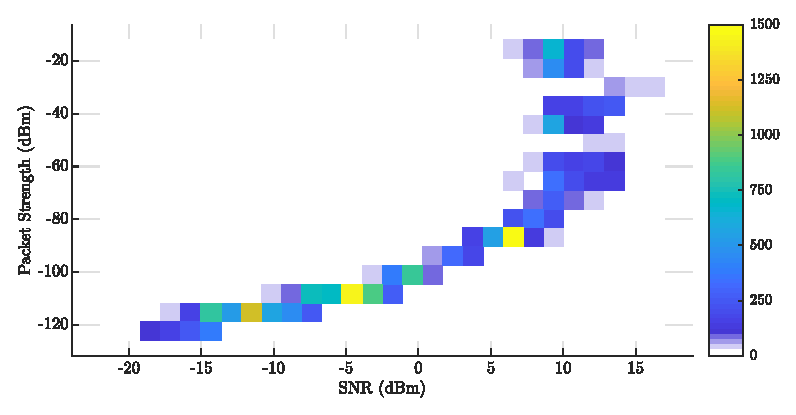
\includegraphics{Figures/density_plot}
    \caption[Test data distribution plot]{
    Density plot of received packet transmissions modelled as a bi-variate histogram with colour indicating received packet count. \\$Total\enskip Points = 19,545$
    }
    \label{fig:density_plot}
\end{figure}

\section{Discussion}
Results are considered in two domains: the demodulation performance of the radio, and the environment effects. This is done because, even though actual receive performance varies with factors such as distance, propagation and fading, these can be abstracted into changes of the underlying \ac{snr} and \ac{ps} figures seen by the receiver. As there are no other transmission sources in this testing, theoretically, if these figures are within the required bounds for demodulation success, the receive will be successful. The demodulation performance is assessed first.

When $\ac{snr} \leq 0$ the \ac{rssi} value indicates the amount of noise seen by the receiver in the presence of no packet. When operating at 868MHz, the noise the receiver should see is approximately the thermal noise floor ($-174+10log_{10}(BW)$), plus the receiver noise figure; \ac{lora} implementations should have a noise figure of around 6dBm [!!!]. This indicates that for a 125kHz receive, the noise floor ($n_f$) should be -117dBm. The empirical noise floor calculated across all locations was -103dBm with a standard deviation of -109dBm; this is 14dBm ($24\times$) higher than expected. As the variance was low, this result indicates that the RFM95W hardware is of much poorer quality than expected, with a noise figure of 20dBm.
\vspace{0.5cm}
\begin{figure}[H]
    \centering
   	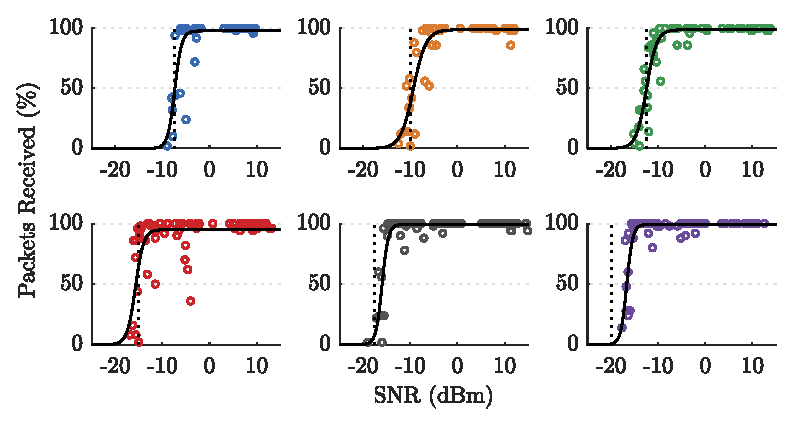
\includegraphics{Figures/sf_pp_separate_plot}
    \caption[Plots of \ac{snr} vs \ac{prp}]{
   \ac{td} mean \ac{snr} values plotted against their \ac{prp}s, separated by \ac{sf}s (Order = [[7, 8, 9], [10, 11, 12]]). For each \ac{sf} plot: the theoretical demodulation limit is indicated by the dotted line and the solid line corresponds to the best-fit sigmoid function; these are repeated in Figure \ref{fig:sf_pp_fit}. Although the best-fit sigmoids give a good representation of the general data pattern, and provide empirical demodulation cut-offs, they do not capture the high-variance receive behaviour when approaching the cut-off. This is reflected by the fact that only 62\%, 60\%, 66\%, 39\%, 77\% and 82\% of the respective training points fall inside the corresponding 95\% confidence interval. Notably \ac{sf}10 has very high-variance; this is reflected in the 95\% maximum receive chance. 
    }
    \label{fig:sf_pp_separate}
\end{figure}

Whether the radio receives a transmission is dictated by whether the received power exceeds the receiver sensitivity ($R_S$). For \ac{lora} modules, $R_S = n_f - \ac{sf}_{lim}$, where $SF_{lim}$ is the minimum SNR required for the current \ac{sf}. Theoretical limits are $-7.5, -10, -12.5, -15, -17.5, -20$ for $\ac{sf} = 7, 8, 9, 10, 11, 12$ respectively. This performance is explored in Figure \ref{fig:sf_pp_separate} and \ref{fig:sf_pp_fit}. In short, performance is close to theoretical for $\ac{sf} = 7, 8, 9, 10$ but $SF=11\enskip \& \enskip 12$ perform similarly to $SF=10$, just with higher reliably. For all configurations, receive success is highly variant when approaching the empirical sensitivity.

\begin{figure}[H]
    \centering
   	\includegraphics{Figures/sf_fit_plot}
    \caption[Plot of sigmoid best-fits for \ac{snr} vs \ac{prp}]{
    Plot of sigmoid best-fits generated in Figure \ref{fig:sf_pp_separate}. The plot clearly demonstrates the positive effect increasing \ac{sf} has on demodulation performance of the receiver. For $\ac{sf}=7,8,9,10$ demodulation success starts dropping approximately 2.5dBm before the theoretical limit ($D_L$), with a 50\% \ac{prp} at $D_L$. This holds less so for \ac{sf}=11, for which drop-off starts around $D_L - 5dBm$, until $D_L$ where there is only a 10\% receive success. For \ac{sf}=12 drop-off starts around $D_L - 7.5dBm$, until $D_L$ where there is a 0\% receive success. Given the stable \ac{rssi} when $\ac{snr} < 0$, and that expected performance holds until a certain \ac{snr}, there is an indication that the sensitivity of the receiver is not as high as stated, possibly due to a cheap hardware implementation.
     }
    \label{fig:sf_pp_fit}
\end{figure}

Theoretically, higher \ac{cr}s will result in more data being recovered from a transmissions allowing for greater receive success. Comparative tests are plotted in Figure \ref{fig:cr_pp_plot}. As no strong visual conclusions can be made, a null hypothesis is proposed; $H_{0} : $ \textit{The mean \ac{prp} does not increase between receives using \ac{cr} 4/5 and \ac{cr} 4/8} (otherwise written as $4/5_{\ac{prp}} \geq 4/8_{\ac{prp}}$). The respective means are 71.8\% and 72.5\%. Using a left-tailed Wilcoxon signed rank test for non-normal distributions, gives $p=41.2\%$. Using a 5\% significance level,  $H_{0}$ cannot be rejected, indicating that \ac{cr} has no effect on \ac{prp}.  Given that the \ac{snr}s are not significantly different \textit{(hypothesis testing omitted)} this indicates that receive drop-off and high variance when approaching sensitivity limits is the limiting factor for demodulation. The lack of \ac{cr} effect is unsurprising given that \ac{fec}'s main performance should be seen in the presence of burst interference.

When the amount of data increases in a packet, its airtime will increase for the same configuration; this can lead to more channel noise being introduced (lower \ac{snr}) and receiver clock drift (lower demodulation performance). The effect this has on comparative tests is plotted in Figure \ref{fig:pl_pp_plot}. The mean \ac{prp}s of $Packet\enskip Length = 20, 128, 255$ are $81.7\%$, $78.8\%$ and $76.8\%$ respectively.  Three null hypotheses are proposed: $H^1_{0} : 20_{\ac{prp}} \leq 128_{\ac{prp}}$, $H^2_{0} : 20_{\ac{prp}} \leq 255_{\ac{prp}}$ and $H^3_{0} : 128_{\ac{prp}} \leq 255_{\ac{prp}}$. Using right-tailed Wilcoxon signed rank tests with 5\% significance, $H^1_{0}$ ($p=1.1\%$) and $H^2_{0}$ ($p=0.0\%$) are rejected but $H^3_{0}$ ($p=13.6\%$) is not. Therefore alternative hypotheses can be accepted  $H^1_{A}=20_{\ac{prp}} \geq 128_{\ac{prp}}$ and $H^2_{A}=20_{\ac{prp}} \geq 255_{\ac{prp}}$. Given that the \ac{snr}s are not significantly different \textit{(hypothesis testing omitted)}, and that $H^3_{A}$ is narrowly rejected, a loose relationship between increased packet length and lower demodulation performance of the receiver is assumed.


\begin{figure}[H]
    \centering
   	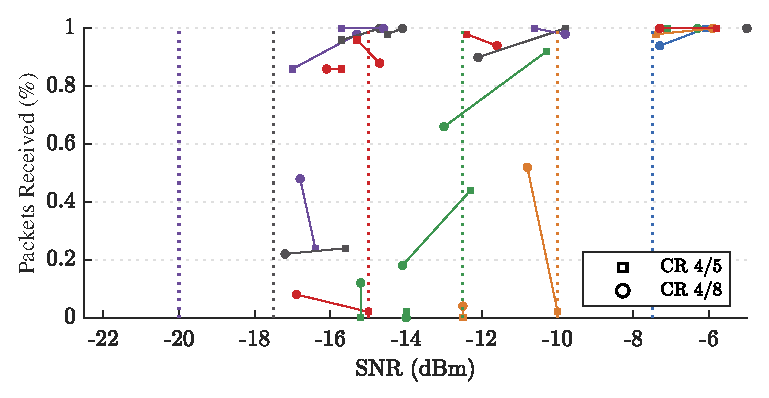
\includegraphics{Figures/cr_pp_plot}
    \caption[Effect of Coding Rate on \ac{snr} and \ac{prp}]{
    Plot of \ac{snr} and \ac{prp} for varying \ac{cr}s. Only configurations where all other factors are identical are included (e.g. height, location, packet length). A line joins each set of points with a matching configuration. \ac{sf} colouring from previous figures is applied to highlight when \ac{snr} limits starts to reduce receive probability. When $SNR > -5$, the \ac{prp} is nearly always 100\% and is therefore excluded. Visual indications are that there is little pattern in the data with 4/5s sometimes outperforming 4/8s and vice versa.
    }
    \label{fig:cr_pp_plot}
\end{figure}

\begin{figure}[H]
    \centering
   	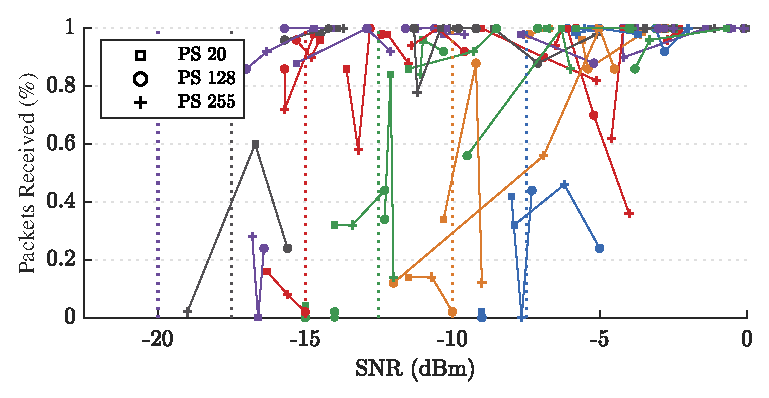
\includegraphics{Figures/pl_pp_plot}
    \caption[Effect of Packet Length on \ac{snr} and \ac{prp}]{
    Plot of \ac{snr} and \ac{prp} for varying packet lengths. Only configurations where all other factors are identical are included. A line joins each set of points with a matching configuration. \ac{sf} colouring from previous figures is applied to highlight when \ac{snr} limits starts to reduce receive probability. When $SNR > 0$, the \ac{prp} is nearly always 100\% and is therefore excluded. Visual indications are that the longer packet lengths have a lower \ac{prp}.
    }
    \label{fig:pl_pp_plot}
\end{figure}

\subsection{Environmental Effects}
\subsubsection{Open (Free) Space}

\subsubsection{Forest}
\subsubsection{Radio Height}
Increasing radio height massively increased range once reached 1m


%Lessons Learnt 
%https://www.thethingsnetwork.org/forum/t/no-lower-rssi-than-121-dbm-possible-in-ttn/19890/15